% https://homepages.inf.ed.ac.uk/rbf/HIPR2/gsmooth.htm
% https://www.wikiwand.com/en/Box_blur
% http://tech.abdulfatir.com/2014/05/kernel-image-processing.html
% https://sbme-tutorials.github.io/2018/cv/notes/4_week4.html#edge-detection-kernels

Gaussian, Box, Passa baixa

\begin{figure}[H]
    \centering
    \begin{subfigure}{0.4\textwidth}
        \centering
        \begin{kmatrix}
    \matrix(img)[square matrix]{
        1 & 4 & 6 & 4 & 1 \\
        4 & 6 & 24 & 6 & 4 \\
        6 & 24 & 36 & 24 & 6 \\
        4 & 6 & 24 & 6 & 4 \\
        1 & 4 & 6 & 4 & 1 \\
    };

    \node[left=of img] {$\displaystyle\Scale[1.7]{\frac{1}{256}}$};
\end{kmatrix}
        \caption{~$h_2$}
        \label{fig:h2}
    \end{subfigure}%
    \begin{subfigure}{0.4\textwidth}
        \centering
        \begin{kmatrix}
    \matrix(img)[square matrix]{
        1 & 1 & 1 \\
        1 & 1 & 1 \\
        1 & 1 & 1 \\
    };

    \node[left=of img] {$\displaystyle\Scale[1.7]{\frac{1}{9}}$};
\end{kmatrix}
        \caption{~$h_6$}
        \label{fig:h6}
    \end{subfigure}

    \caption{Máscaras de \textit{blur}.}
    \label{fig:blur:kernel}
\end{figure}

\begin{figure}[H]
    \centering
    \begin{subfigure}{0.48\textwidth}
        \centering
        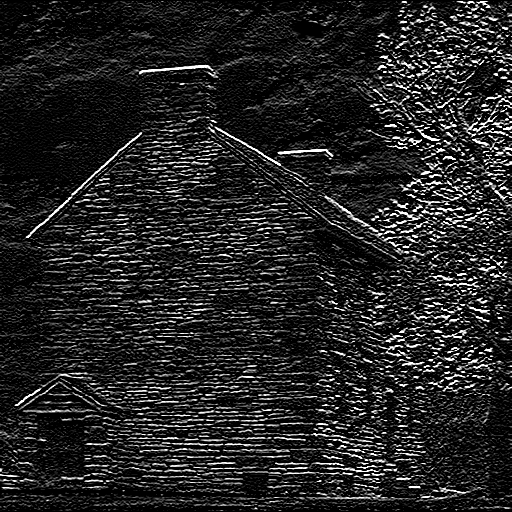
\includegraphics[width=0.9\textwidth]{imagens/house.png}
        \caption{Original: \texttt{house.png}.}
    \end{subfigure}\\[8pt]
    \begin{subfigure}{0.48\textwidth}
        \centering
        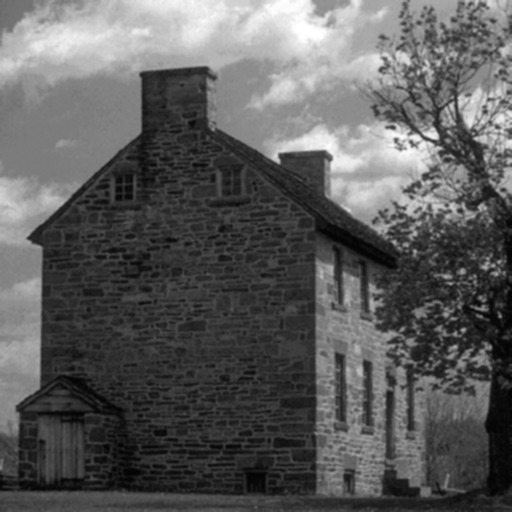
\includegraphics[width=0.9\textwidth]{resultados/house_h2.png}
        \caption{Convolução com $h_2$ (\ref{fig:h2}).}
    \end{subfigure}%
    \begin{subfigure}{0.48\textwidth}
        \centering
        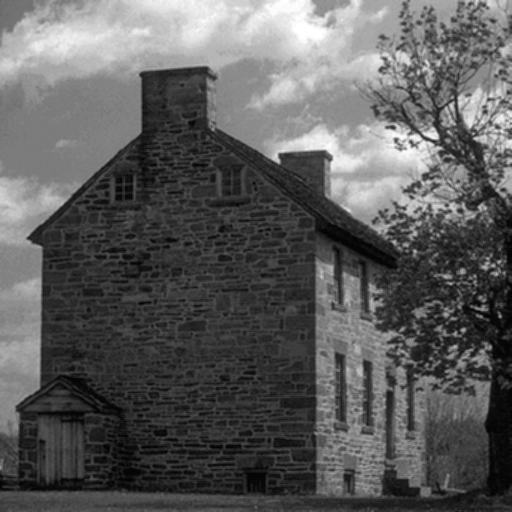
\includegraphics[width=0.9\textwidth]{resultados/house_h6.png}
        \caption{Convolução com $h_6$ (\ref{fig:h6}).}
    \end{subfigure}

    \caption{Aplicação do \textit{blur}.}
    \label{fig:blur}
\end{figure}
